% fig_67_margin.tex
% TR-32: Directional criterion value vs k_ibr for 67N and 67Q (forward + reverse)
%
% X-axis: k_ibr [0.02, 0.20] pu
% Y-axis: criterion value Re[-V_seq * conj(I_seq)] [pu^2]
%
% 67N forward  (green)  : ~0.030 to 0.049 pu^2 (I0 from network, ~constant)
% 67N reverse  (red)    : ~-0.030 to -0.049 pu^2
% 67Q forward  (blue)   : proportional to k_ibr^2 * R1S
% 67Q reverse  (orange) : negative
%
% I_min_67 = 0.04 pu (dashed vertical line)
% I_min_21 = 0.10 pu (dashed vertical line)
% Zero line: thick grey
%
% Data (alpha=0.50, X/R=20):
%   67N fwd: value = Re[Z0S]*|I0(alpha=0.5)|^2 = 0.015 * 1.598^2 ≈ 0.03830
%            constant w.r.t. k_ibr (I0 independent)
%   67Q fwd: value = Re[Z1S]*k_ibr^2 = 0.005 * k_ibr^2
%            k=0.02: 0.000002  k=0.04: 0.000008  k=0.10: 0.000050  k=0.20: 0.000200

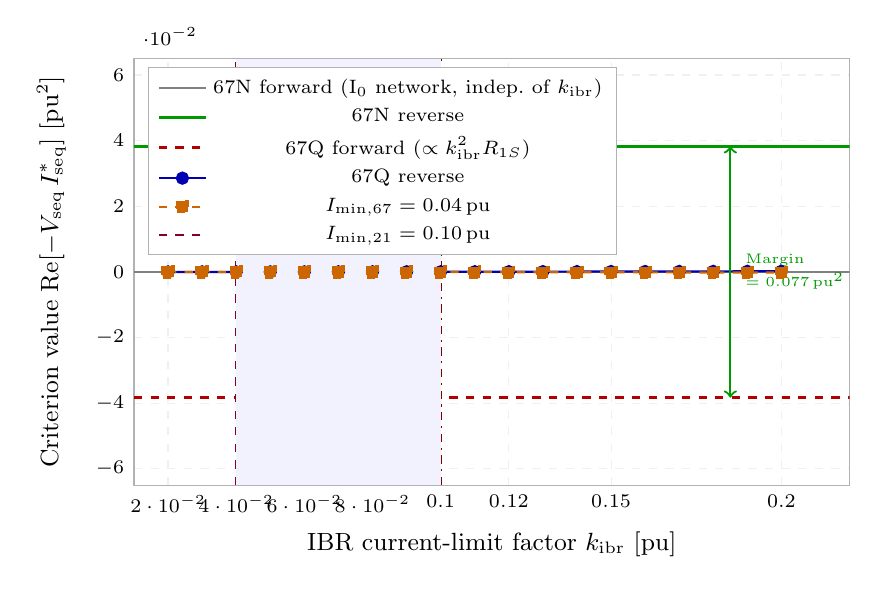
\begin{tikzpicture}
\begin{axis}[
  name         = margax,
  width        = 0.88\textwidth,
  height       = 7.0cm,
  xlabel       = {IBR current-limit factor $k_\mathrm{ibr}$ [pu]},
  ylabel       = {Criterion value $\mathrm{Re}[-V_\mathrm{seq}\,I_\mathrm{seq}^*]$ [pu$^2$]},
  xlabel style = {font=\small},
  ylabel style = {font=\small, yshift=4pt},
  xmin=0.01, xmax=0.22,
  ymin=-0.065, ymax=0.065,
  xtick        = {0.02,0.04,0.06,0.08,0.10,0.12,0.15,0.20},
  xticklabel style={font=\scriptsize},
  yticklabel style={font=\scriptsize},
  legend style={at={(0.02,0.98)}, anchor=north west, font=\scriptsize,
                draw=gray!60, fill=white},
  grid         = major,
  grid style   = {gray!12, dashed},
  tick style   = {draw=none},
  axis line style={gray!60},
]

%% ── Zero line ─────────────────────────────────────────────────────────────
\addplot[black!50, thick, mark=none]
  coordinates {(0.01,0) (0.22,0)};

%% ── 67N forward (constant wrt k_ibr) ─────────────────────────────────────
\addplot[green!60!black, very thick, mark=none]
  coordinates {(0.01,0.03830) (0.22,0.03830)};
\addlegendentry{67N forward (I$_0$ network, indep.\ of $k_\mathrm{ibr}$)}

%% ── 67N reverse ────────────────────────────────────────────────────────────
\addplot[red!70!black, very thick, mark=none, dashed]
  coordinates {(0.01,-0.03830) (0.22,-0.03830)};
\addlegendentry{67N reverse}

%% ── 67Q forward (proportional to k_ibr^2) ────────────────────────────────
\addplot[blue!70!black, thick, mark=*, mark size=2pt,
         domain=0.02:0.20, samples=19]
  ({x}, {0.005*x*x});
\addlegendentry{67Q forward ($\propto k_\mathrm{ibr}^2 R_{1S}$)}

%% ── 67Q reverse ────────────────────────────────────────────────────────────
\addplot[orange!80!black, thick, mark=square*, mark size=2pt,
         domain=0.02:0.20, samples=19, dashed]
  ({x}, {-0.005*x*x});
\addlegendentry{67Q reverse}

%% ── I_min thresholds ────────────────────────────────────────────────────────
\addplot[purple!70!black, thick, dashed, mark=none]
  coordinates {(0.04,-0.065) (0.04,0.065)};
\addlegendentry{$I_\mathrm{min,67}=0.04$\,pu}

\addplot[red!50!black, thick, dash dot, mark=none]
  coordinates {(0.10,-0.065) (0.10,0.065)};
\addlegendentry{$I_\mathrm{min,21}=0.10$\,pu}

%% ── Annotation: 67Q coverage zone ──────────────────────────────────────────
\fill[blue!5] (axis cs:0.04,-0.065) rectangle (axis cs:0.10,0.065);
\node[blue!50!black, font=\tiny, align=center]
  at (axis cs:0.07, 0.050)
  {67Q covers\\21 blocked};

%% ── Annotation: 67N margin ─────────────────────────────────────────────────
\draw[<->, green!60!black, thick]
  (axis cs:0.185, 0.03830) -- (axis cs:0.185, -0.03830);
\node[green!60!black, font=\tiny, right=2pt, align=left] at (axis cs:0.185, 0)
  {Margin\\[1pt]$= 0.077$\,pu$^2$};

\end{axis}
\end{tikzpicture}
